\chapter{LSP features}
\section{Highlighting}
The HLASM Language Support extension highlights statements with different colors for labels, instructions, operands, remarks and variables. Statements containing instructions that can have operands are highlighted differently to statements that do not expect operands. Code that is skipped by branching AIF, AGO or conditional assembly is not colored.

\begin{figure}[h]
	\centering
	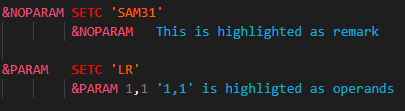
\includegraphics[width=10cm]{img/highligting}
	\caption{An example of highlighting.}
\end{figure}

\section{Autocomplete}
Autocomplete is enabled for the instruction field. While typing, a list of instructions starting with the typed characters displays. Selecting an instruction from the list completes it and inserts the default operands. Variables and sequence symbols are also filled with a value from their scope.

\begin{figure}[H]
	\centering
	\animategraphics[autoplay,loop,width=\linewidth]{12}{img/autocomplete/autocomplete-}{0}{126}
	\caption{\href{https://github.com/eclipse/che-che4z-lsp-for-hlasm/blob/master/readme\_res/autocomplete.gif}{Autocomplete usage example.}}
\end{figure}

\section{Go To Definition and Find All References}
The extension adds the \TT{go to definition} and \TT{find all references}' functionalities. Use the \TT{go to definition} functionality to show definitions of variable symbols, ordinary symbols and macros, or open COPY files directly. Use the \TT{find all references} functionality to show all places where a symbol is used.
	
\begin{figure}[H]
	\centering
	\animategraphics[autoplay,loop,width=\linewidth]{12}{img/go_to_def/go_to_def-}{0}{90}
	\caption{\href{https://github.com/eclipse/che-che4z-lsp-for-hlasm/blob/master/readme\_res/go\_to\_def.gif}{Go To Definition usage example.}}
\end{figure}
	

